\chapter{Testing with Whisker}
\label{cha:appraoch}

\section{General Approach}
\label{sec:general_appraoch}

In this work, we propose a way to perform dynamic testing on Scratch programs for Scratch 3.0.
The main goal of this approach is to be able to automatically assess student's solutions to Scratch assignments.
In order to do so, this approach makes use of an automation utility, which allows test code to
interact with Scratch programs through Scratch's IO.
\parspace

Because Scratch's parallel scripts, as well as its lack of code separation, would make testing individual parts of programs difficult,
we instead chose to test full programs on the level of system tests, and only focus on the program's input and output.
This raises the question of how to access Scratch's IO.
Since its input usually consists of mouse and keyboard input, and its output consists of visual animations and sound,
the IO is not easily accessible in a programmable way.
To overcome this challenge, we developed an automation utility called Whisker, which acts as a wrapper around Scratch.
It interacts with Scratch's virtual machine in order to automate its input and output.
Whisker offers a programmable interface for Scratch, which allows tests to simulate inputs and to access information about sprites and variables.
This makes automated testing for Scratch possible.
Figure~\ref{fig:comparison_of_io_mechanisms} illustrates the difference between Scratch's IO mechanisms and Whisker's automated input and output.
Note that the current version of Whisker does not yet support audio output or Scratch's extensions.

\begin{figure}[htpb]
    \centering

    \begin{subfigure}[b]{\textwidth}
        \centering
        \tikzset{>=latex,
               arrow/.style={draw, -{Latex[length=1.5mm, width=1.5mm]}},
                 put/.style={draw, minimum height=1.7cm, minimum width=3.5cm, rounded corners, fill=red!20, text width=2.5cm, text centered},
                  vm/.style={draw, minimum height=3.0cm, minimum width=6.0cm, rounded corners, fill=white},
                 gui/.style={draw, minimum height=4.2cm, minimum width=7.0cm, rounded corners, fill=blue!20},
                 box/.style={draw, minimum height=4.2cm, minimum width=4.0cm, rounded corners, text width=3.5cm},
              boxtxt/.style={minimum width=4.0cm, rounded corners, text width=3.5cm}}

         \begin{tikzpicture}[scale=0.8, every node/.style={scale=0.8}]
            \begin{scope}[on background layer]
                \node[gui] at (0.0,  0.4) (gui)     {};
                \node[vm]  at (0.0,  0.0) (vm)      {};
            \end{scope}

            \node[put]     at (0.0, -0.4) (put)     {\textbf{Program under test}};
            \node[]        at (0.0,  1.0) (vmtxt)   {\textbf{Scratch Virtual Machine}};
            \node[]        at (0.0,  2.0) (guitxt)  {\large \textbf{Scratch GUI}};
            \node[box, left=of gui]       (input)   {};
            \node[box, right=of gui]      (output)  {};
            \node[boxtxt, below right] at ([yshift=-2mm] input.north west)  (inputtxt)
                {\centering {\large \textbf{Input}}\\[.5\baselineskip]Key presses, mouse movement, mouse clicks, etc.};
            \node[boxtxt, below right] at ([yshift=-2mm] output.north west) (outputtxt)
                {\centering {\large \textbf{Output}}\\[.5\baselineskip]Visual animations, audio, etc.};

            \path [arrow] (input) -- (gui);
            \path [arrow] (gui)   -- (output);
        \end{tikzpicture}
        \caption{Input and output of the Scratch GUI}
    \end{subfigure}

    \bigskip

    \begin{subfigure}[b]{\textwidth}
        \centering
        \tikzset{>=latex,
               arrow/.style={draw, -{Latex[length=1.5mm, width=1.5mm]}},
                 put/.style={draw, minimum height=1.7cm, minimum width=3.5cm, rounded corners, fill=red!20, text width=2.5cm, text centered},
                  vm/.style={draw, minimum height=3.0cm, minimum width=6.0cm, rounded corners, fill=white},
             whisker/.style={draw, minimum height=4.2cm, minimum width=7.0cm, rounded corners, fill=green!20},
                 box/.style={draw, minimum height=4.2cm, minimum width=4.0cm, rounded corners, text width=3.5cm},
              boxtxt/.style={minimum width=4.0cm, rounded corners, text width=3.5cm}}

         \begin{tikzpicture}[scale=0.8, every node/.style={scale=0.8}]
            \begin{scope}[on background layer]
                \node[whisker] at (0.0,  0.4) (whisker) {};
                \node[vm]      at (0.0,  0.0) (vm)      {};
            \end{scope}

            \node[put]         at (0.0, -0.4) (put)     {\textbf{Program under test}};
            \node[]            at (0.0,  1.0) (vmtxt)   {\textbf{Scratch Virtual Machine}};
            \node[]            at (0.0,  2.0) (guitxt)  {\large \textbf{Whisker}};
            \node[box, left=of whisker]       (input)   {};
            \node[box, right=of whisker]      (output)  {};
            \node[boxtxt, below right] at ([yshift=-2mm] input.north west)  (inputtxt)
                {\centering {\large \textbf{Input}}\\[.5\baselineskip]Simulated user inputs through a programmable interface};
            \node[boxtxt, below right] at ([yshift=-2mm] output.north west) (outputtxt)
                {\centering {\large \textbf{Output}}\\[.5\baselineskip]Interface to access information about sprites and variables};

            \path [arrow] (input)   -- (whisker);
            \path [arrow] (whisker) -- (output);
        \end{tikzpicture}
        \caption{Input and output of Whisker}
    \end{subfigure}

    \caption{Comparison of IO mechanisms between the Scratch GUI and Whisker}
    \label{fig:comparison_of_io_mechanisms}
\end{figure}

\section{Testing Environment}
\label{sec:testing_environment}

Whisker is, like Scratch 3.0, implemented in JavaScript (JS).
Hence, test code is also written in JavaScript.
Whisker can theoretically be used with any JS testing framework,
but for compatibility reasons, we developed a simple testing framework to go along with Whisker.
\parspace

Currently, Whisker is only available in its own web GUI, which can be seen in Figure~\ref{fig:whisker_gui}.
The web page displays Scratch's stage, a table of loaded tests, and a test report in TAP13\footnote{Test Anything Protocol, \url{https://testanything.org/}} format.
It supports batch testing more than one program with the same test suite,
but it doesn't support parallel test execution.
In the future, we plan on implementing a standalone Electron\footnote{\url{https://electronjs.org/}} application for Whisker.
This would facilitate batch testing many programs,
and would also make it possible to test programs in parallel.
Unfortunately it is not possible to run tests in a headless environment,
because Scratch depends on a HTML canvas to render its output to.
Without a renderer, some of Scratch's blocks don't work properly.

\begin{figure}[htpb]
    \centering
    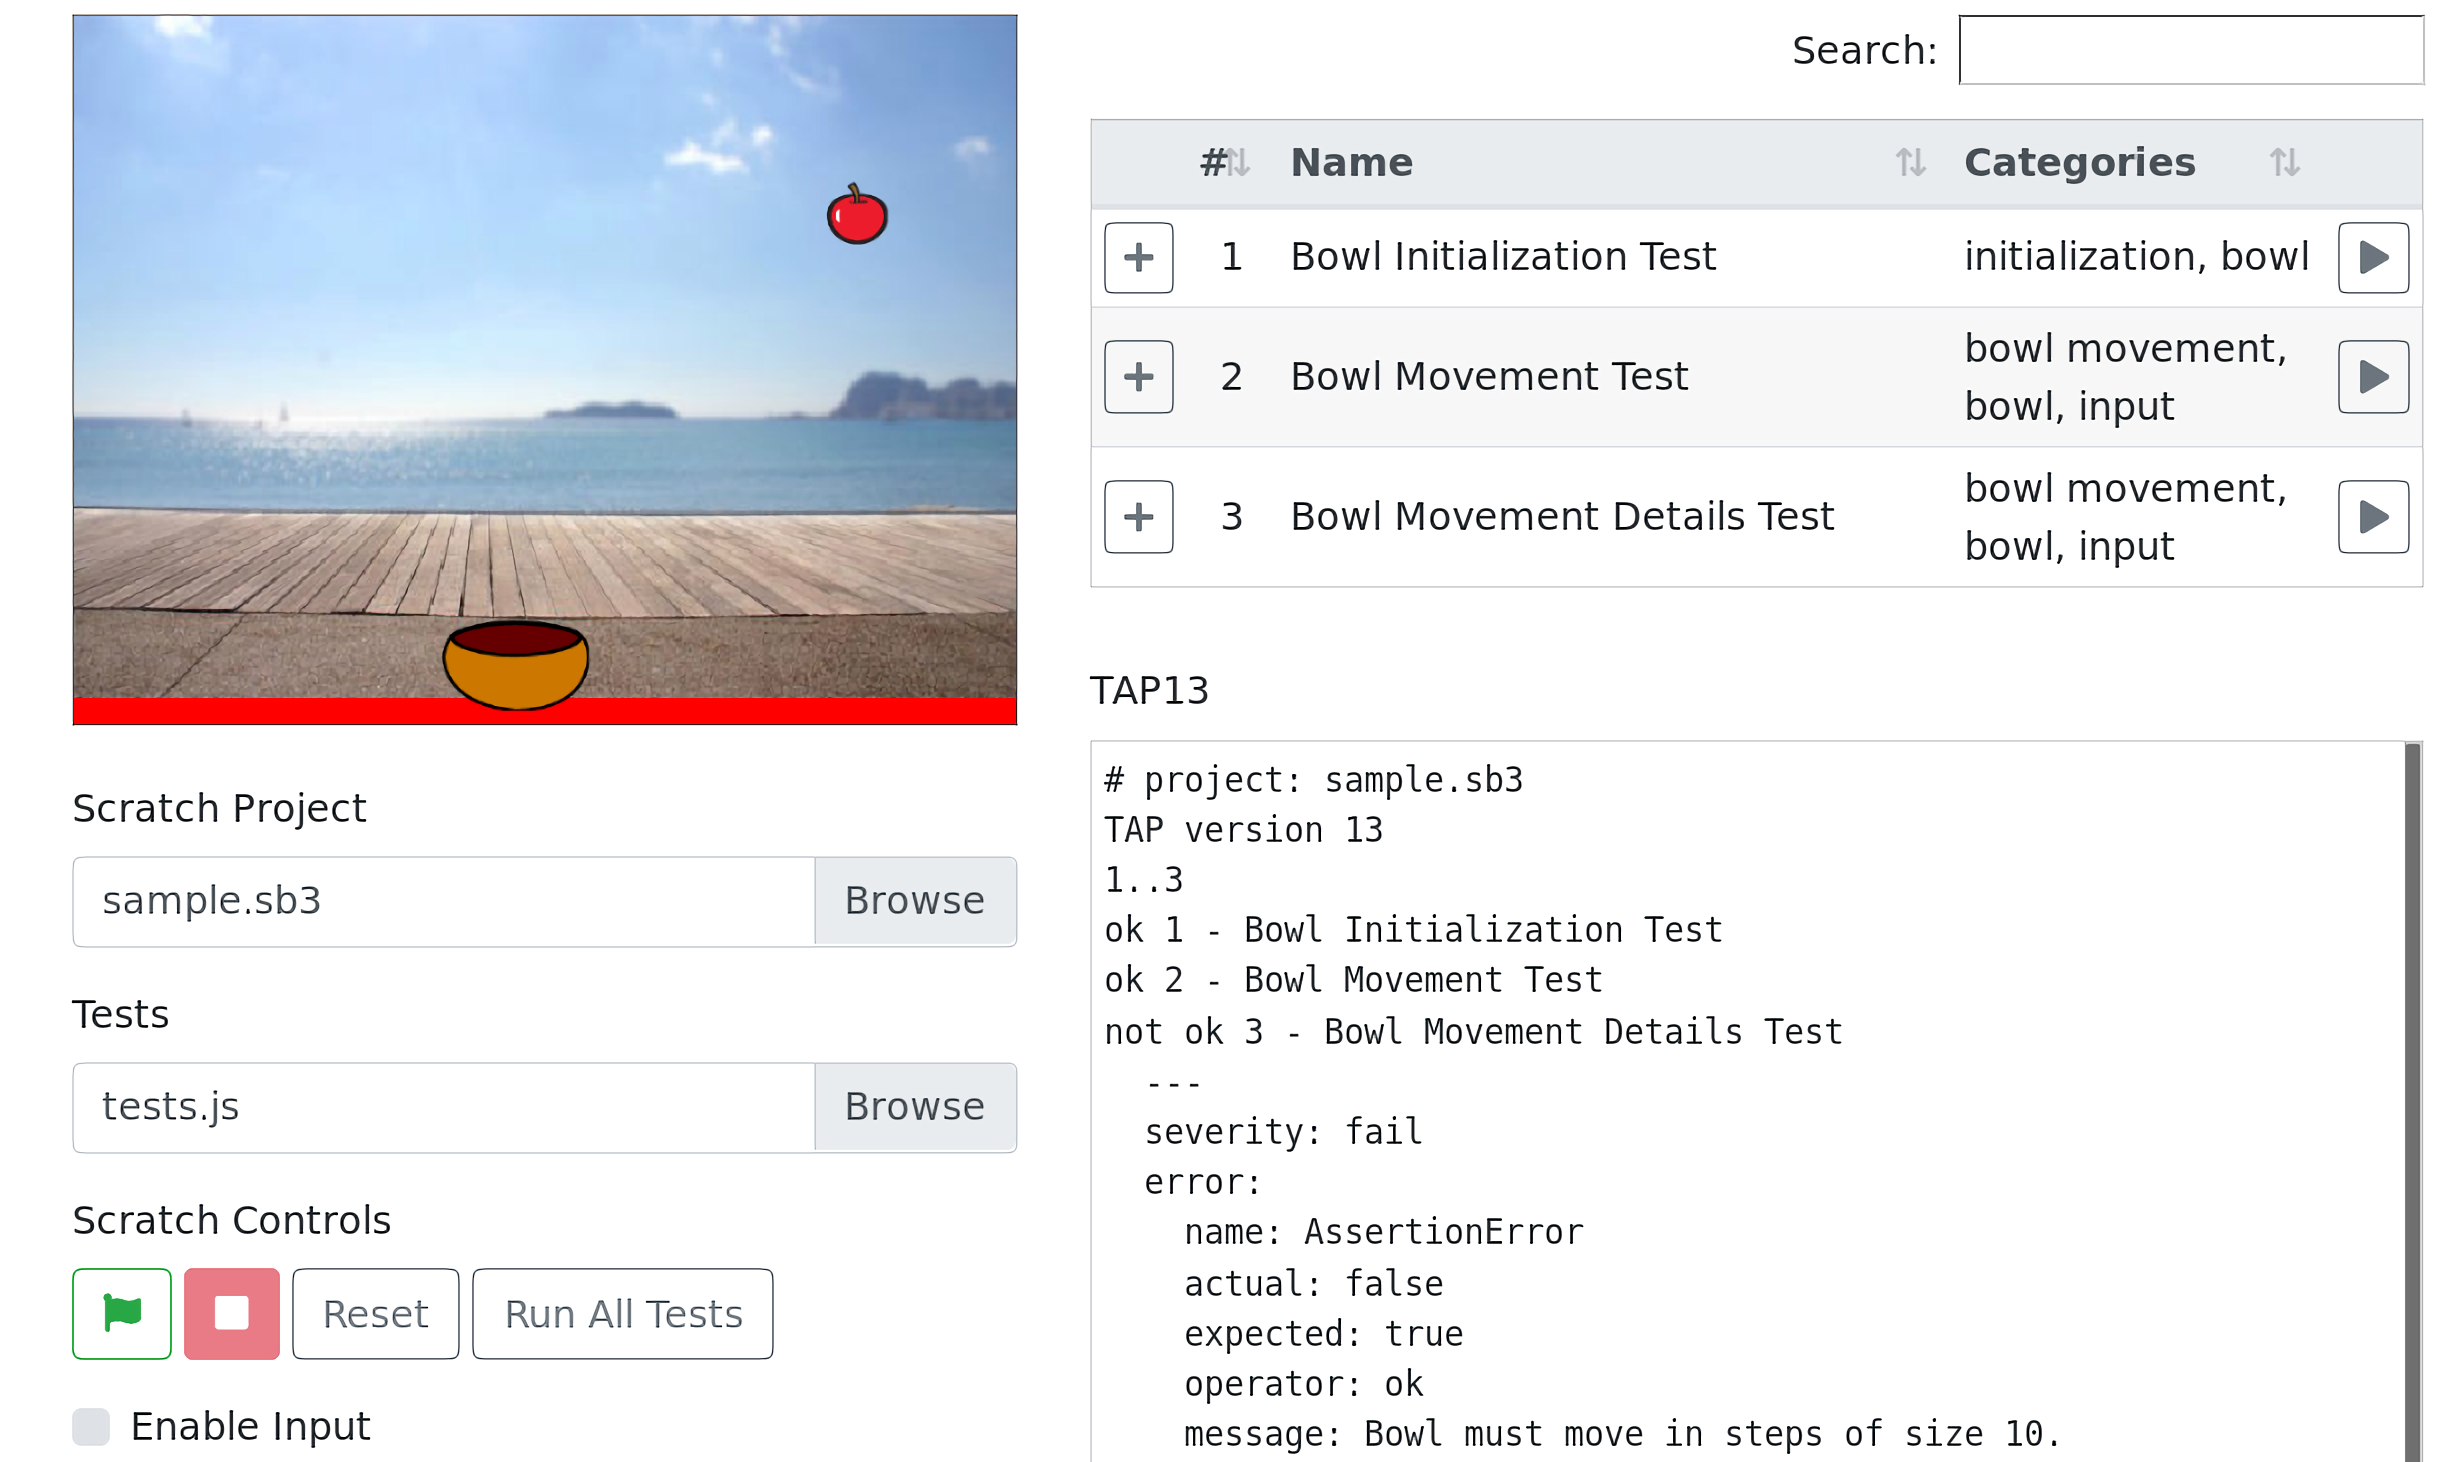
\includegraphics[width=.95\textwidth]{whisker-gui-big-upscaled}
    \caption{Whisker's web interface}
    \label{fig:whisker_gui}
\end{figure}

\section{Whisker's Public Interface}
\label{sec:public_interface}

Tests use a test driver object to automate Scratch through Whisker.
Whisker's own testing framework automatically passes the test driver object to its tests as an argument,
but tests written for other testing frameworks may have to acquire the test driver in their test code.
Whisker offers an interface to create and configure the test driver object for this purpose.
Listing~\ref{fig:examples_of_how_to_acquire_the_test_driver} shows code examples for both possibilities.
Whisker loads the program before each test case in order to create the same initial state for every test,
instead of going on where the last execution left off, like Scratch's GUI does it.
It also starts the program with the green flag when the test begins.

\begin{listing}[htpb]
    \centering
    \begin{subfigure}[b]{.35\textwidth}
        \begin{minted}[autogobble, breaklines, linenos, fontsize=\scriptsize, framesep=2mm, frame=lines]{javascript}
            async function test (t) {
                ...
            }
        \end{minted}
        \vspace{-\bigskipamount}
        \caption{Getting the test driver passed as a parameter}
    \end{subfigure}
    \hspace{.05\textwidth}
    \begin{subfigure}[b]{.50\textwidth}
        \begin{minted}[autogobble, breaklines, linenos, fontsize=\scriptsize, framesep=2mm, frame=lines]{javascript}
            async function test () {
                const whisker = new WhiskerUtil(vm, project);
                whisker.prepare();
                const t = whisker.getTestDriver();
                whisker.start();
                ...
            }
        \end{minted}
        \vspace{-\bigskipamount}
        \caption{Manually acquiring the test driver through Whisker's interface}
    \end{subfigure}
    \caption{Acquiring the test driver}
    \label{fig:examples_of_how_to_acquire_the_test_driver}
\end{listing}

The following list will give an overview of Whisker's basic functions.
Because Whisker is still in early development, some of its methods may undergo changes later.
The test driver object will be denoted as $t$ in example code snippets.

\begin{itemize}
    \item \textbf{Control the program execution.}
        Tests are able to control when and for how long the program under test is run.
        In the beginning of the test, the program starts in a paused state.
        The program can then be run (resumed) for a certain amount of time, or until a condition is met.
        Since the Scratch program execution is asynchronous, we use JavaScript's Promise API for this purpose.
        In order to simply execute the program and wait until the execution is done, the test can be declared as an \texttt{async function} and use the \texttt{await} keyword.

        The green flag can also be pressed again in order to restart the program.
        Additionally, tests can query the currently elapsed time,
        either from the start of the last program execution,
        or from the start of the test case.
        \begin{javascriptcode}
            /* Run the program for one second (1000 ms or 30 steps). */
            await t.runForTime(1000);
            await t.runForSteps(30);

            /* Run the program until a condition is met, or until one second elapsed.
             * The condition is given by a function that returns a boolean. */
            await t.runUntil(() => a > b, 1000);

            /* Get the total time elapsed in the current / last run. */
            t.getRunTimeElapsed();

            /* Get the total time elapsed in this test case. */
            t.getTotalTimeElapsed();

            /* Press the green flag again. */
            t.greenFlag();
        \end{javascriptcode}
    \item \textbf{Simulate Inputs.}
        By simulating Scratch's main input methods, tests can control the program under test.
        The goal is to simulate a user interacting with the program.
        The possible input includes mouse movement, mouse button presses, keyboard key presses, and entering answers to \texttt{ask} blocks.
        Inputs, that press (or release) a key or button, can specify a duration, after which the key is released (or pressed) again.
        Inputs can be performed immediately, or registered to be performed after a delay during the next execution.
        Inputs, that aren't performed during a run, will still trigger hats that respond to the input.
        Tests can also query the current mouse position and if a certain key or button is pressed.

        Note that inputs, that press a key for a long duration, do not issue multiple key press events.
        Usually, when holding down a key, the operating system repeats that key press,
        which will trigger "when key is pressed" hats repeatedly.
        This is not the case for simulated input.
        However, keys can be simulated to be released and instantly pressed again,
        which will trigger "when key is pressed" hats.
        \begin{javascriptcode}
            /* Perform a keyboard input immediately. */
            t.inputImmediate({
                device: 'keyboard',
                key: 'right arrow',
                isDown: true,
                duration: 100 // time in ms
            });

            /* Perform a mouse input one second into the next run. */
            t.addInput(1000, { device: 'mouse', x: 100, y: 200, isDown: true });

            /* Answer an ask block two seconds into the next run. */
            t.addInput(2000, { device: 'text', text: 'some answer' });

            /* Query the current state of the inputs. */
            t.getMousePos(); // {x, y}
            t.isMouseDown();
            t.isKeyDown('space');
        \end{javascriptcode}
    \item \textbf{Access Scratch's output.}
        Whisker provides access sprites and variables of the program.
        They are accessed through sprite and variable objects, which always have the latest attributes of the sprite or variable they reference.
        Sprite objects can be obtained by their name or by their attributes.
        The provided sprite attributes include the sprite's position, rotation, size, current costume, speech bubble text, etc.
        Sprites also include the attribute values from the previous Scratch execution step,
        which can be accessed through the \texttt{old} attribute of the sprite objects.
        Additionally, sprites offer methods for detecting collisions, and other helper methods.
        \begin{javascriptcode}
            /* Get a sprite by its name. */
            const sprite = t.getSprite('Sprite1');
            /* Get sprites that match a condition. */
            const sprites = t.getSprites(sprite => sprite.x > 100);
            /* Get a sprite's clones. */
            const clones = sprite.getClones();
            /* Get the stage. */
            const stage = t.getStage();

            /* Various getter methods for variables. */
            const variable = stage.getVariable('my variable');
            const variables = stage.getVariables();
            const list = sprite.getList('my list');
            const lists = sprite.getLists();

            /* Accessing sprite attributes and variable values.
             * Sprites and variables always have the latest values.
             * sprite.old has the values from the previous execution step. */
            sprite.x;
            sprite.old.x;
            variable.value;

            /* Some of the helper methods. */
            sprite.isOriginal();
            sprite.isTouchingEdge();
            sprite.isTouchingSprite(otherSprite);
        \end{javascriptcode}
    \item \textbf{Register Callbacks.}
        Tests can execute code during the program execution by registering callbacks, which get called every time Scratch executes a step.
        Callbacks can be registered to be executed before or after each step execution.
        This allows tests to react to information, which the user would normally see, while the program is running.
        Callbacks can, for example, be used to track information, to perform inputs according to sprite information, or to cancel a run.
        Callbacks can be enabled and disabled.
        \begin{javascriptcode}
            /* Add a callback to be called before each step. */
            const callback = t.addCallback(() => {
                if (sprite.x > 100) {
                    t.inputImmediate({ device: 'mouse', isDown: true });
                } else if (sprite.x < 0) {
                    t.cancelRun();
                }
            });

            /* Add a callback to be called after each step (true as 2nd parameter). */
            t.addCallback(() => someList.push(sprite.x), true);

            /* Enable / disable a callback, check if a callback is active. */
            callback.disable();
            callback.enable();
            callback.isActive();
        \end{javascriptcode}
    \item \textbf{React to sprite movements and visual changes.}
        In addition to callbacks, which get called before or after each Scratch program step,
        tests can also set a function to be called whenever a sprite moves, or whenever a sprite's visuals change.
        The function takes the changed sprite as a parameter.
        This can be useful for detecting events, that happen during the step, but are not displayed to the user,
        which is needed for some edge cases.
        For example, consider program with two scripts:
        One of the scripts moves a sprite around.
        The other script moves the sprite back to the center of the screen whenever it touches on of the stage's edges.
        Therefore, whenever the sprite touches an edge, it is immediately moved back to the center,
        even before the image is rendered.
        A normal callback will never detect the sprite touching an edge,
        but this way, detecting these collisions is possible.
        \begin{javascriptcode}
            let touchedEdge = false;

            t.onSpriteMoved(sprite => {
                touchedEdge = touchedEdge || sprite.isTouchingEdge();
            });

            t.onSpriteVisualChange(sprite => { /* ... */ });
        \end{javascriptcode}
    \item \textbf{Register constraints.}
        By registering constraints, tests can define conditions that must always hold.
        Constraints are realized through special callbacks, which perform one or more assertions.
        Whisker can be configured to fail the test on a constraint failure (the default) or to simply disable the failed constraint.
        In the second case, it is up to the test code to check which constraints failed and react accordingly.
        \begin{javascriptcode}
            /* Configure the action taken when a constraint fails. */
            t.onConstraintFailure('fail');
            t.onConstraintFailure('nothing');

            /* Register a constraint to check if some sprite is always visible. */
            const constraint = t.addConstraint(() => {
                t.assert.ok(sprite.visible === true, 'Sprite must always be visible.');
            });

            /* Enable / disable a constraint, check if a constraint is active. */
            constraint.disable();
            constraint.enable();
            constraint.isActive();
        \end{javascriptcode}
    \item \textbf{Perform randomly generated inputs.}
        Whisker provides random input generation by performing a randomly chosen input from a pool of possible inputs
        in a specified interval during program executions.
        Tests can either provide the pool or inputs to choose from themselves
        or they can let Whisker determine what inputs the program reacts to through static analysis.
        If a input consists of multiple events (i.e.\ if it has a duration) the same input cannot be chosen again while still active.
        If all of the inputs in the pool are active, no random inputs are performed until at least one input is done.

        Inputs in the pool can specify intervals for their attributes,
        from which a value is randomly chosen when the input is performed.
        They can also be assigned a weight to make them more likely or less likely to be chosen.
        \begin{javascriptcode}
            /* Set the interval. A random input is performed every 150ms
             * during program execution. */
            t.setRandomInputInterval(150);

            /* Register random inputs for the pool manually. */
            t.registerRandomInputs([
                  { device: 'keyboard', key: 'left arrow', duration: [50, 100] },
                  { device: 'keyboard', key: 'right arrow', duration: [50, 100] },
                  { device: 'mouse', x: [-100, 100], y: [-100, 100], weight: 0.5 }
            ]);

            /* Let Whisker detect inputs for the pool. */
            t.detectRandomInputs({ duration: [50, 100] });
        \end{javascriptcode}
\end{itemize}
\parspace

\section{Challenges of this Approach}
\label{sec:appraoch_challenges}

This section highlights various challenges that one can face when using this approach to aid in grading Scratch assignments.%
\parspace

\textbf{General testing challenges.}
Firstly, automated testing in general introduces some challenges.
For one thing, programs have to be well specified, since testing relies on the program's specification.
Therefore, if the specification is too vague, testing can become difficult.
Tests for imprecise specifications potentially need to consider more possible cases of how the program could behave.
Likewise, conflicting interpretations of the specification between the test and the program may result in false negative test outcomes.
Also, since the program is only tested as a whole, testing a single part of the program can be difficult.
If some feature of the program under test depends on another feature being implemented correctly,
but the latter does not work, the first feature can not be tested properly.
\parspace

\textbf{Addressing sprites and variables.}
In order to access information about sprites and variables, they need to be addressed in some way.
Sprites can be addressed by their name or by any of their attributes, for example by their position.
Nevertheless, if a sprite, that is needed for the test, can not be found, the test can not work properly.
This can be a problem if a Scratch program deviates from the specification.
For example, if students are given a template with sprite names already in place,
some students could rename the sprites, causing tests to fail.
However, errors like this can easily be detected through test reports.
\parspace

\textbf{Missing initialization.}
Another challenge are programs with missing initialization which are saved in a bad state.
When the green flag is pressed, the Scratch GUI simply picks up where the last execution left off.
Therefore, students might not initialize their program properly,
which can cause it to sometimes behave incorrectly when the green flag is pressed.
A program with missing initialization may be saved in a bad state,
meaning the program will behave incorrectly the next time it is started.
Since we restore the same state in the beginning of each test case,
such a program will always behave incorrectly during the tests although the implementation might be mostly correct.
\parspace

\textbf{Parallel initialization.}
Since Scratch runs all ''when green flag is pressed'' scripts in parallel,
programs tend to mix their initialization with actual program execution.
This may make it difficult to test initialization,
since some initialized values may already change while others have not been initialized yet,
meaning that the program is never in a clean initialized state.
\parspace

\textbf{Time-displaced events.}
Programs may have events that are supposed to trigger certain actions.
For example, a sprite touching another sprite may cause a variable to be incremented.
But the exact timing for the triggered action is often unknown, because the event is detected through a loop.
Therefore, tests have to check if the action happens in a time interval after the event occurred.
This may be done by tracking timestamps of the event and the action, and comparing these timestamps,
but this can be expensive to do.
